\documentclass[12pt]{article}
\usepackage[a4paper,left=2cm, right=2cm, top=2cm, bottom=2cm]{geometry}
\usepackage{amssymb}
\usepackage{amsmath,mathtools}
\usepackage{relsize}
\usepackage{epsfig,graphicx}
\usepackage{color}
\usepackage{xcolor}
\usepackage{tikz}
% \usepackage{subfigure}
\usepackage{hyperref}
\usepackage{algorithm}
\usepackage{algorithmic}
\usepackage{cite}
\usepackage{amsfonts}
\usepackage{textcomp}
\usepackage{xcolor}
\usepackage{multirow}
\usepackage{authblk}
\usepackage{subcaption}

\begin{document}

% \def\BibTeX{{\rm B\kern-.05em{\sc i\kern-.025em b}\kern-.08em
%  T\kern-.1667em\lower.7ex\hbox{E}\kern-.125emX}}

\title{Route Optimization For Waste Collection\\}
\date{}
\author[1]{Marut Priyadarshi}
\author[2]{Meet Maratha}
\author[3]{Mohammad Anish}
\author[4]{Vaibhav Kumar}
\affil[1]{Department of Data Science Engineering, IISER Bhopal}
\affil[2]{Department of Data Science Engineering, IISER Bhopal}
\affil[3]{Department of Physics, IISER Bhopal}
\affil[4]{Department of Data Science Engineering, IISER Bhopal}

\maketitle

\section{Introduction}

Solid Waste Management (SWM) is considered one of the critical drivers of urban environmental management systems \cite{hoornweg2012waste}.It is generally an exercise to collect the combined waste from households, agricultural industrial, commercial activity, institutional, and miscellaneous, generated from the living community \cite{GUPTA2015206}. India is one of the least urbanized countries in the world, yet urban India produces about 42.0 million tons of municipal solid waste annually, i.e., 1.15 lakh metric tons per day (TPD) \cite{SHARMA2021293,GUPTA2015206}. These figures are bound to increase in the future, as cities are witnessing extreme demographic transfers, immigration, population growth, and consumption rate, which are the key driving factors for the increase in urban waste. This has become one of the most urgent concerns for local agencies in India. During the last decade, the government has launched various programs e.g., Clean India Mission, Smart Cities, Amruth Cities, and Digital India to improve living standards. Waste management is one of the core infrastructure elements of these missions, which requires empirically driven conclusions to address the SWM related challenges \cite{CHEELA2021419}. 

Solid waste collection is the most integral activity of SWM. However, the waste collection in India is very unorganized, primarily due to resource constraints and poor planning of available resource \cite{somani2021integrated,GUPTA2015206}. Collection vehicle route planning (VRP) is the major resource component of a waste collection system, whose planning is often not driven by analytics, resulting in poor collection efficiency \cite{akbarpour2021innovative}. Similar scenarios have been reported by in almost every city in developing countries \cite{GUPTA2015206}. VRP requires modeling many components such as path planning, consideration of available resources, spatiotemporal demand patterns, and real-time dynamics of waste volume at collection points and trucks. A plethora of literature addresses subsets of these components in solution development. However, a holistic waste collection system that considers them simultaneously for any region has not been reported in the literature \cite{han2015waste}. Hence, the onground implementation of the present approaches are still very limited. This significantly impacts the operation costs and, eventually, the environment \cite{apaydin2007route}. Moreover, the components and their interrelationships are very complex for the resource-constrained societies, and therefore pose new challenges that require the researchers' urgent attention.

To address the challenges stated above, we propose a waste collection framework for cities, with the objective to find the optimal routes for the available vehicle paths while considering the dynamic variations in the waste information at collection points and also that of the vehicles. We also discuss the influence of available resources in covering the collection bins, whose dynamic information drives the best path. Finding the best path is formulated as an optimization problem and solved using linear programming. The approach has an advantage over other traditional path planning approaches due to the considerations of field-based activities in the model. Further, the study  focuses on resource-constrained societies resulting in a decision making tool that can be scaled and applied universally with the following major contributions:

\begin{itemize}
\item Analysis of truck availability in study regions on waste collection, to demonstrate the total coverage.
\item Consideration of quantitatively simulated dynamic waste levels for truck and
collection bins for realistic outcomes.
\item Detailed sensitivity analysis of various parameters affecting selection of the best path.
\end{itemize}

\section{Related Studies:}

There has been a decent amount of work done in different aspects of waste collection, such as the costs, route optimization, smart bins, segregation, landfill and collection depot optimal locations. But, by far, the most common topic of work in this area has been VRP and, in recent years, Internet of Things (IoT) enabled smart designs for the waste management systems. 

Optimization of vehicle routes is one of the main objectives for this paper. VRP has been previously approached from many directions such as landfill and collection sites allocation to minimize distance traveled by collection vehicles \cite{kulcar1996optimizing,rathore2020location,barzehkar2019landfill}, collection point clustering to increase collection efficiency \cite{al2021optimization} and calculating the optimal route with a fixed set of collection nodes and landfill/depot locations \cite{karadimas2008routing, amal2018sga, asefi2019mathematical,de2007decision, hannan2020waste,akhtar2017backtracking}. The mathematical calculations of the VRP have been solved through pre-existing route optimizer software, such as the ArcGIS Network Analyst \cite{karadimas2008routing,amal2018sga, malakahmad2014solid}, or a formulated single or multi objective functions that calculate the desired routes \cite{hannan2020waste,de2007decision}. The biggest drawbacks of these models is that they are predominantly static and calculate the optimal routes once for a set of collection points. Even the papers that do focus somewhat on dynamic methods, they are mostly theoretical and lack the elements necessary for real life application \cite{hannan2020waste}. Some studies have further incorporated smart bins with the VRP to develop a more robust and resource efficient solution to the optimization problem \cite{akhtar2017backtracking,lozano2018smart,baldo2021multi}. These utilize IoT enabled smart bins to keep track of the waste that needs to be collected and reduce redundancy in waste collection runs. Most of these models focus on case studies set in developed nations, which are not constrained in terms of resources.

The application of route optimization models in resource constrained societies is the second of our main objectives. Waste collection in resource constrained societies comes with the additional challenge of having to allocate insufficient resources to meet the demands as much as possible. While not as many as before, there have been papers that focus on this aspect of waste collection \cite{chaudhary2019gis,rathore2020location,sk2020optimal,malakahmad2014solid, ogwueleke2009route}. The study in \cite{chaudhary2019gis} utilizes ArcGIS Network Analyst to calculate optimal waste collection routes in the city of Allahabad. While it does take real life data of collection and landfill sites into consideration for the route calculation, it relies on a pre-existing route optimizer to get the final results.\cite{ogwueleke2009route} and \cite{malakahmad2014solid} focus on route optimization in the cities of Onitsha, Nigeria and Ipoh City, Malaysia respectively. The paper \cite{rathore2020location} focuses on optimal node allocation to maximize the waste collection in the city of Bilaspur, India. These works, however, do not consider any real time data to calculate the optimal routes. This is one of the things this paper seeks to address.

There have been many more works done in the field of VRP and the papers mentioned above are in no way exhaustive. They were just meant to be indicative of the general direction of the research done in this field. There are a number of excellent reviews that go into much more detail regarding the other works that address optimization of waste collection and management systems \cite{belien2014municipal,sulemana2018optimal,abdallah2020artificial}. The engineering and construction aspects of the smart bins are outside the scope of this paper, however other works have delved into much more detail on this problem \cite{vishnu2021iot,lozano2018smart}.


% In one paper \cite{kulcar1996optimizing}, the author focuses on the best location for the construction of a landfill that would result in the shortest collection routes when linked with the currently existing routes and depots. The paper also compares the running costs of different modes of waste transport, such as trains, ships and by road. It was useful in providing a picture of the costs associated with the system, it didn't focus on optimizing the routes that the waste collection was done. Moreover, it was set in Brussels, a highly developed city. In a similar vein, Rathore et al. \cite{rathore2020location} focuses on formulating a mathematical model for finding the optimal places to allocate bins in the Indian city of Bilaspur. While it aims towards the similar goal of waste collection optimization, furthermore in a developing country, the method is different from our intended goal.

% Many papers utilize pre-existing solvers or software to compute the optimized routes and use the results to compare them to other algorithms or observe the effects the optimized routes bring to the current system. In the case of one paper \cite{karadimas2008routing}, the sole focus of the paper is on route optimization. However, it only applies ant colony system and the route optimizer for the software ArcGIS Network Analyst to get the optimal route for non-real time data and compares the efficiencies of the two methods. Moreover it focuses on Athens, another developed city, and even then on only one prefecture of it. Similarly, Chaudhary et al \cite{chaudhary2019gis} have utilized ArcGIS Network Analyst software to calculate optimal routes for waste collection, this time in the city of Allahabad. This lies closer to our goal of route optimization for more resource constrained societies and while it is an extensive application of optimization process utilizing the real-life data from the city, it still only utilizes a pre-existing algorithm along with fixed unchanging datapoints to calculate the collection routes, which our work seeks to expand upon. Another paper \cite{amal2018sga} uses the route optimization solver of GIS software ArcGIS (which itself utilizes Dijkstra algorthm) to calculate a pool of routes which, in turn, feeds the genetic algorithm to iteratively arrive at the optimal routes for the waste collection vehicles.

% In their paper, Simonetto and Borenstein \cite{de2007decision}, used linear programming to formulate a function for route optimization via minimization of cost coupled with a heuristic developed by Renaud and Boctor \cite{renaud2002sweep} in order to bring down the computation time (at that time) to reasonable levels. Similarly, in this paper \cite{hannan2020waste}, the authors have used linear programming combined with smart bins to find optimal waste collection routes that remove the inefficiency that is associated with formulating a route that visits all nodes, regardless of its fill status. However, as it was a paper focused on the algorithmic part of the problem, they used purely simulated data, void of any real world analogue and only factored in the euclidian distances between the nodes. Asefi et al \cite{asefi2019mathematical} uses a mixed-integer linear programming model to minimize costs and uses two different meta heuristic approaches to deal with the non-deterministic polynomial-time hardness of the waste collection problem. This model is then applied to a case study in the city of Tehran, Iran. 

% In other papers utilizing smart bins, Akhtar \cite{akhtar2017backtracking} utilizes new population based meta heuristic backtracking search optimization, developed by Civicioglu \cite{civicioglu2013backtracking}, to calculate optimal routes for collection vehicles. Its main feature is its simplicity as it has only one control parameter. It is also a highly theoretical work and focuses mainly on the mathematical aspects of the problem and not its real-life application. Al-Refaie et al \cite{al2021optimization} takes a different approach and focuses instead on distributing the collection points into optimal clusters so that the collection efficiency of the vehicles can be maximized.

% Papers like Lozano et al \cite{lozano2018smart} and later Baldo et al \cite{baldo2021multi}, Vishnu et al \cite{vishnu2021iot} use smart bins, but the focus of these papers are the smart bins themselves, their engineering aspect and case studies involving them, along with constructing a system centered around technology which automates a lot of the tasks involved in the whole process of waste collection and management. The optimization part is left to pre-existing solving algorithms.

% Smart bins have also been discussed in a more theoretical aspect, utilizing IoT technology in other studies such as Abdullah et al \cite{abdullah2018iot}, Ali et al \cite{ali2020iot}, Al-Masri et al \cite{al2018serverless} and Chaudhari and Bhole \cite{chaudhari2018solid}. They have touched upon smart bins as parts of a sustainable smart city architecture and different ways that they may be utilized, along with supporting subsystems. It should be noted that the above-cited literature is in no way an exhaustive list of literature utilizing IoT or smart bins, and merely provides a general idea of the works using it.

Our model integrates the concept of smart bins with the optimization algorithm. Smart bins are simply bins that are connected to the internet and provide real time data on how full they are. This data is used by the model to calculate new optimal routes for the collection vehicles after a specified time interval, based on the real-time locations of the vehicles. This paper's main priority is to create a model for route optimization that is suitable for a resource constrained city, yet is general enough to be scaled to fit more developed societies. Moreover, our model works with real time data, capable of adapting to new data and calculating new routes based on changing information, and that information is gained through smart bins. This paper also seeks to keep the simulated data as close the real life situations as possible so that the gap between theory and implementation would be minimal.

\section{Problem Definition and Mathematical Formulation}


\subsection{Problem Definition}
We address the problem of developing a vehicle routing model by minimizing the incurred travel cost and maximizing the waste collected by the vehicles considering various real-time considerations. We have considered an Indian city to demonstrate its outcomes. To implement the model we have divided the study area in various regions. The region consists of collection bins which are used to collect waste and generally caters a large areas. These bins as nodes are assumed to be located on a road network made from edges and nodes. We simulated temporally varying waste values for each of these bins, we call them "smart bins". The simulation helped us in overcoming the requirement of physical sensor placement at these locations. We incorporated the inputs of stakeholder agency in the simulation purpose to keep the simulation values closer to the actual scenarios. 
	
A collection vehicle is assigned to a region only collects waste from bins from a specific region through an optimal route.  The "route" in our problem corresponds to path of the vehicles covering these bins and finishing its trip at a depot. The path is made up of  non-directional edges. To make the implementation realistic we have applied limits on the total waste that can be collected by the vehicles. 
The numerical values of the distances are normalized to the same scale as the waste values to avoid any skewness. The model is executed after a certain time interval by considering  bins waste values, vehicle waste fill status, vehicle location,  and generates a route which keeps updating with the time. We implemented the smart bins in the route finding process using a priority queues where priority is being given to a bin based on the distance to that bins and the amount of waste value of bin, that is, for the same distance value, the bin with the greater waste value is assigned higher priority. The model stops when either the run is complete or the vehicle is full. \textcolor{red}{A "time slice" here is the route calculation that is done for one time interval, which is repeated multiple times with updated data to get the final route. The "run" in our problem signifies the whole process of calculating the route for one vehicle, beginning and ending at the depot. A run is the aggregate of multiple time slices over time.} The values of the bins can be updated even when the vehicle is moving on an edge and hasn't reached the next node. For such scenarios the model assumes that the vehicle has completed the current edge and considers the next node as the starting point for the new time slice.

\textcolor{red}{While running the optimization process, each individual bin is randomly assigned a value between 0 and 1 to denote how full the bin is. This value is updated with each time slice to simulate the real life accumulation of waste in bins. When transferring waste from the bins to the truck, a conversion factor is used to convert the waste amount from the percent fill ratio of the bin to the percent fill ratio of the truck. The trucks are programmed to run in parallel, that is, each truck starts its collection run at the same time and continues until they reach full capacity. If a truck, in one time slice, does not visit a node, if there is sufficient capacity remaining, one of the other trucks will address that node.}

Three different execution scenarios are demonstrated. The first scenario restricts the available resources, which in our case is the collection vehicles. The second case demonstrates the impact of available resources on waste collection, bins covered and distance travelled for each region and accumulated at city scale. Lastly we emphasize the importance of dynamic consideration by comparing the outcome of dynamic model with the static model.

\subsection {Mathematical Formulation}

The objective of the model is to maximize the waste collected while minimizing the total distance travelled by the vehicles. We formulate the model as a mixed integer linear programming problem and solved it using Gurobi optimizer \cite{gurobi} in polynomial time. Such solvers can solve problems with realistic instance sizes, which was in our case.

In our problem, our two main objectives are:
\begin{itemize}
    \item Minimize the distance travelled by the collection vehicles
    \item Maximize the waste collected through the collection run
\end{itemize}

The following table defines all the variables used for the mathematical formulation:
\begin{table}[H]\label{variables}
	\centering
	\caption{The description of variables}
	\begin{tabular*}{486pt}[H]{|c|c|}
		\hline \hspace{40pt} Variables \hspace{40pt} & \hspace{130pt} Description \hspace{130pt} \\
		\hline i, j & Node i and Node j respectively.\\
		\hline N & Nodes for a particular truck excluding depot.\\
		\hline D & Nodes for a particular truck including depot.\\
		\hline \multirow{2}{*}{A} & Set of all the arcs formed from a\\
		&  node i to a node j for $\forall$ i,j $\in$ V.\\
		\hline \multirow{2}{*}{$C_{ij}$} & Distance cost from a node i\\
		& to a node j for a truck.\\
		\hline \multirow{2}{*}{$X_{ij}$} & It is a binary variable that is 1 if a truck is\\
		& travelling between the node i and node j.\\  
		\hline \multirow{2}{*}{$Y_{i}$} & It is a binary variable that is 1 if a truck is \\
		& visiting node i.\\
		\hline \multirow{2}{*}{$u_{i}$} & The percentage fill of the truck at node i \\
		& following given path, for a specific time slice.\\
		\hline \multirow{1}{*}{st} & The starting node of a truck in a\\
		& new time slice.\\
		\hline \multirow{2}{*}{$w_{1}$} & The weight assigned to the distance \\
		& objective of the objective function\\
		\hline \multirow{2}{*}{$w_{2}$} & The weight assigned to the waste amount \\
		& objective of the objective function\\
		\hline \multirow{1}{*}{$f_{i}$} & The fill ratio of bin at node i.\\
		\hline \multirow{2}{*}{$BT$} & The conversion factor for fill \\
		& of smart bin to fill of truck.\\
		\hline \multirow{1}{*}{$P_{t}$} & Cumulative fill percentage of truck at a time slice t.\\
		\hline
	\end{tabular*}
\end{table} 

With this we can formulate our base objective function to be:

\begin{equation}\label{eq1}
    Obj(minimize)=\sum_{i,j \in A} w_1 X_{ij} C_{ij} - w_2 Y_i f_i * BT
\end{equation}

Here, $X_{ij}$ is a binary variable that can only take the values 0 or 1, based on the fact whether a truck took a route from i to j or not. $C_{ij}$ is the cost, or the distance travelled when moving from i to j. $Y_{i}$ is another binary variable that indicates if waste from node i has been collected or not. $BT$ is the conversion factor of how much would the waste from a node would fill up a truck collecting it. $f_i$ represents the fill ratio (the percentage of how full the bin is) of the bin, its value being between 0 and 1. 0 meaning it is empty and 1 meaning it is full. The variables $w_1$ and $w_2$ are the weights associated with distance travelled and waste collected, respectively, to determine which attribute of waste collection should have the higher priority and by how much. \textcolor{red}{A single instance of the objective function is defined for one vehicle, but for the route optimization involving multiple trucks, multiple instances of the objective function, one for each vehicle, is ran in parallel to simulate simultaneous runs of collection vehicles in real life.}

For the weights $w_1$ and $w_2$ the following constraint applies:

\begin{equation}\label{eq1.5}
    \sum_{n\in \{1,2\}} w_n = 1
\end{equation}

That is, the total sum of $w_1$ and $w_2$ will always remain equal to 1. This will be later used to perform the weight analysis in order to get the optimal ratios of the weights for our objective function.

For the objective function to fully represent our problem, we need to add constraints. The subscript 'st' denotes the starting node at the start of another time slice after the given time interval.
\begin{equation}\label{eq2}
    \sum_{j\in N}X_{st,j}=1 ; \forall st \in N ; j \in N
\end{equation}
\begin{equation}\label{eq3}
    \sum_{j\in N}X_{j,st}=1 ; \forall st \in N ; j \in N
\end{equation}
Node 0 is assigned to be the depot, the start and the end point of every collection run. Eq (\ref{eq2}) and Eq (\ref{eq3}) ensure the looping of the route, with the added caveat that since the calculations are made multiple times per run (called time slices) as new data is obtained, the value of the starting node for each subsequent time slice, after the initial one, changes. Therefore, these new starting nodes have to also be taken into consideration.
\begin{equation}\label{eq4}
    \sum_{i\in N}\sum_{j\in D } X_{ji}=1 ; \forall i,j \in A ; j\ne i
\end{equation}
\begin{equation}\label{eq5}
    \sum_{i\in N}\sum_{j\in D } X_{ij}=1 ; \forall i,j \in A ; j\ne i
\end{equation}
Eq \eqref{eq4} and Eq \eqref{eq5} specify that the nodes that are already visited by the truck in a collection run are not considered again for for further calculations, or in simpler terms, a node that has already been visited is not visited again in the same run.

The variable $u_i$ is a temporary variable that resets to zero at the beginning of each time slice. It represents the percent the the truck is full for each separate calculation. Variable $P_t$ is the variable that stores all the cumulative progress of how full the truck is, in percent, over all the previous and subsequent time slice.

If:
$$ X_{ij}=1$$
then:
\begin{equation}\label{eq7}
    u_i+f_j*BT =u_j ; \forall i,j \in A 
\end{equation}
for: 
$$ i,j\ne 0$$
$$ i,j \ne st $$
This constraint (Eq \eqref{eq7}) ensures that if a truck goes on an arc (an arc being a small portion of the entire collection route) from two consecutive nodes, node i to node j, the amount of waste is continuous, that is, the waste in the truck at node j is the sum of the waste at node i and the waste collected in the route i to j. The value of the waste inside the truck is updated at node j so that there is no discrepancy in the case when a new path has to be calculated with new data.
\begin{equation}\label{eq8}
    u_i\ge f_i*BT
\end{equation}
$$  \forall i\in N$$
Eq \eqref{eq8} ensures that the amount of waste in a truck after reaching a node must be greater than or equal to the waste it had before that. This makes sure that the truck is actually collecting the waste from that node and not just passing it.
% Added this equation
\begin{equation}\label{eqY}
	\sum_{i\in N}Y_i f_i* BT\le100-P_t
\end{equation}
Eq \eqref{eqY} ensures that the truck will not collect waste from a node if collecting from that node makes the truck exceed its maximum capacity. Therefore, for the sake of maximizing waste collected, such nodes will not be taken into consideration for further time slices.
\begin{equation}\label{eq12}
    u_i\le 100 - P_t
\end{equation}
$$\forall i \in N $$
This constraint in Eq \eqref{eq12} ensures that for a single time slice in the collection run, the value of how full the truck is does not exceed its capacity. Since $P_t$ stores the cumulative fill percentages of the truck, in any subsequent and previous time slices, the fill percent of the truck should not exceed the sum of the previous fill percentage and the percent filled in the current calculation. 

With this, we have formulated our problem and now we can move on to implementing and calculating the solution for our problem

\section{Case Studies and Empirical Results}

\subsection{Data Preparation}

To prove the effectiveness of the model, we empirically tested the model for the city of Chandigarh in India. The city is located by the foothills of the Shivalik range of the Himalayas in northwest India. It covers an area of approximately 114 km$^2$. It borders the states of Punjab and Haryana. The city is known for being the first planned city of India. The city also has various scattered unplanned built-up patches such as Burail, Nayagaon. The mixed built-up typology was suitable to test the methodology. Hence, the city was found suitable to test the methodology. We generated various waste collection points (location of smart bins) for the city. A total of 300 points were generated randomly using Geographic Information System (GIS) functionalities, with the constraint that the point should fall on the road networks. The road network was extracted from Open Street Map (OSM) database. OpenStreetMap API was then used to calculate the distance between all nodes, and generate a distance matrix which was used in the optimization process. We applied K-Means clustering algorithm to cluster these points in a fixed set of clusters (see Figure 1). In this paper we have selected total clusters to be three. The number can be updated based on user requirements. After clustering, region1, region2 and region3 had 95, 111 and 94 points, respectively. The clusters were considered as three regions for which vehicles had to be allocated. To replicate the actual field activities we have considered that a vehicles starts and ends its route at the depot (see Figure) \ref{figm})


\begin{figure}[H]
    \centering
    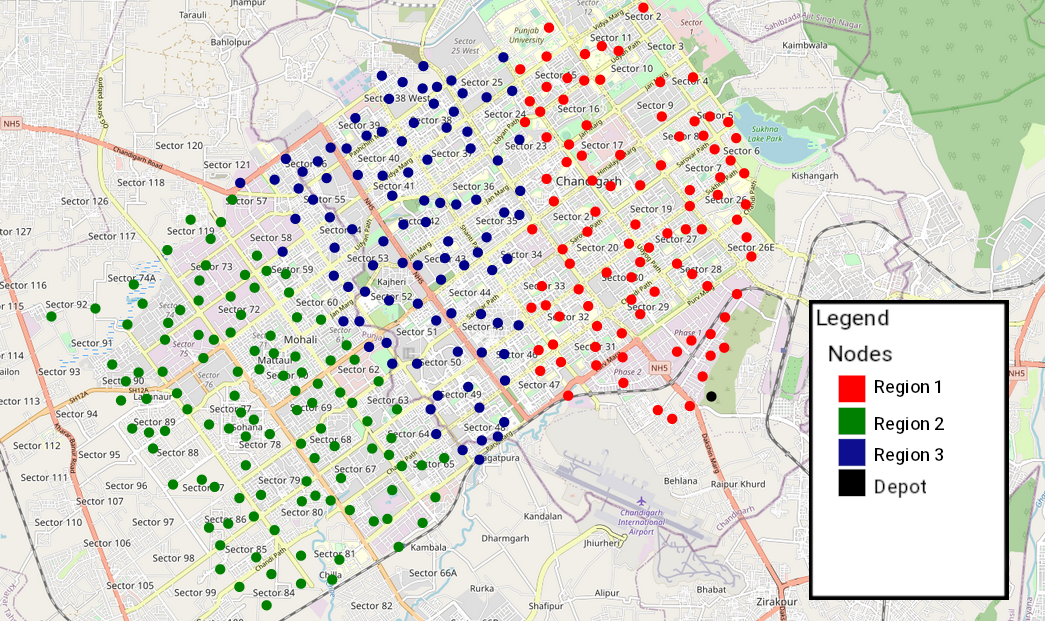
\includegraphics[scale=0.4]{Nodes.png}
    \caption{The selected nodes and their clusters}\label{figm}
\end{figure}

\subsection{Execution case studies}
Experiments were carried out on a AMD A6-9220 processor which runs at 2.5GHz and utilizes 8 GB RAM. The model was implemented in Python 3.10.5 and solved with Gurobi optimizer version Gurobi 9.5.1. A total of four scenarios were implemented and the minimum and maximum solving time was around 67.0618 s having total variable count: 7041 and total constraint count: 7075 for the maximum case.

As per Dengel et al \cite{degel2015time}, one of the most common approaches to handle multi-criteria decision problems is the weighted sum approach. In this approach, the objectives are aggregated prior to the optimization by assigning weights to the objective functions. The weights are based on the decision makers preference in order to model the importance of the goal, which in our case is to find minimum path route while maximizing the collected waste. 

The suggestion of the decision makers (Municipal Corporation Chandigarh) was to provide equal preference to find minimum distance routes and maximizing the waste collection. hence, we assigned  $w_1$ and $w_2$ to be 0.5 to execute the scenarios. This means that our optimization model gives equal importance to minimizing the distance and maximizing the waste collected. To highlight the important of weights a detailed sensitivity analysis of weights on outcomes is discussed later in a subsection.
The maximum available number of collection vehicles (mv) was considered to be 7, and was considered same for all the regions. The values are selected based on the input of the decision makers. The maximum capacity of a truck (TC) was considered as 1000 Kg, and the maximum capacity of a smart bin (BC) was considered as 100 Kg.

\subsubsection*{Case 1: Restriction on Resources}
To highlight the importance of strategical usage of available resources in resource constraint societies, we applied restrictions on the available collection vehicles. The vehicle values were varied from one to six and the impact on total distance travelled, total waste collected, and total nodes covered was studied for each region, and  eventually for the city. The routes were calculated while considering the temporal dynamics of bin and waste level, truck positions in varying time-steps. Table \ref{tab1} illustrates the cumulative values for the distance and wastes outcomes for all the trucks in each region.
\begin{table}[H]
    \centering
    \caption{Data for the real-time restricted case} \label{tab1}
    \vspace*{0.3cm}
    % Following are the changes
    \hspace*{-1cm}
    \begin{tabular}{|c|c|c|c|c|c|c|}
        \hline \multirow{2}{*}{Case} & \multicolumn{2}{c|}{Region 1} & \multicolumn{2}{c|}{Region 2} & \multicolumn{2}{c|}{Region 3}\\
        \cline{2-7}& Waste (Kg)  & Distance (Km) & Waste (Kg) & Distance (Km) & Waste (Kg) & Distance (Km)\\ 
        \hline \textit{1 Truck} & 999.89 & 39.79 & 997.36 & 63.11 & 999.94 & 59.22 \\
        \hline \textit{2 Trucks} & 1992.68& 99.58 & 1994.29 & 129.37 & 1984.23& 119.51 \\
        \hline \textit{3 Trucks} & 2989.61 & 142.05 & 2997.77 & 195.04 & 2979.87 & 180.71 \\
        \hline \textit{4 Trucks} & 3989.43 & 208.59 & 3986.17 & 279.63 & 3977.46 & 241.80 \\
        \hline \textit{5 Trucks} & 4961.06 & 321.16 & 4966.69 & 345.68 & 4964.88 & 322.97 \\
        \hline \textit{6 Trucks} & 5282.82 & 362.89 & 5959.62 & 433.19 & 5179.85 & 373.26 \\
        \hline
    \end{tabular}
\end{table}

A significant impact of available trucks on collected waste can be observed. Further, the increase in waste collected for different number of trucks per region varied linearly for each region to the total distance traveled by all the trucks (Figure \ref{figz}). The increase in distance and collected waste is a direct result of having more trucks running at the same time. For region1 and region3, a sharp drop in the waste collected was observed after five trucks. Which means almost all the smart bins for these regions was catered by these trucks. On the other hand region2 still required more resources to cater the demand. This is more evident by Table \ref{tab3}, which details the case of 6 trucks per region to determine whether it is sufficient to satisfy the waste collection demand of regions and the city. It can be observed all bins for regions 1 and 3 were covered by utilizing 6 trucks, while only 85\% of the nodes for region2 were covered by the six trucks. This is primarily because the value of waste for the bins in this regions was higher due to region2 having more nodes than region1 and region3.

\begin{figure}[H]
    \centering
    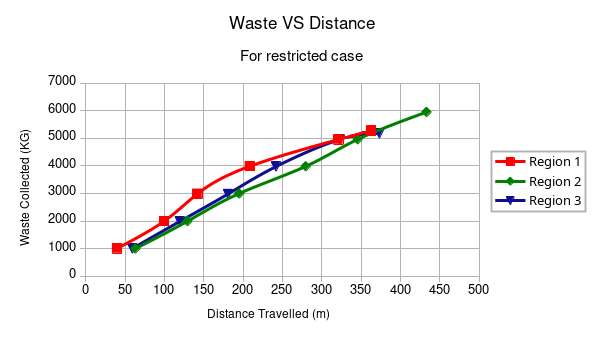
\includegraphics[scale=0.6]{distance_VS_garbage_restricted.png}
    \caption{Distance traveled vs waste collected}\label{figz}
\end{figure}


\begin{table}[H]
    \centering
    \caption{ Data for 6 trucks per region} \label{tab2}
    \vspace*{0.3cm}
    % Changed Values
    \begin{tabular}{|c|c|c|c|c|c|}
        \hline Region & Truck & Waste (Kg) & Distance (Km) & Waste/Distance & Percent collected \\
        \hline \multirow{4}{*}{Region 1} & Truck 1 & 999.07& 38.53 & 25.93 &14.7368\% \\
        \cline{2-6}& Truck 2 & 990.67 & 47.20 & 20.99 & 13.6842\%\\        
        \cline{2-6}& Truck 3 & 994.66 & 43.57 & 22.83 & 15.7895\%\\        
        \cline{2-6}& Truck 4 & 998.21 & 72.55 & 13.76 & 20.0000\%\\      
        \cline{2-6}& Truck 5 & 977.66 & 121.86 & 8.02 & 24.2105\%\\      
        \cline{2-6}& Truck 6 & 322.56 & 39.19 & 8.23 & 11.5789\%\\
        \hline & & & &\textbf{Total:} &\textbf{100\%}\\
        \hline \multirow{4}{*}{Region 2} & Truck 1 & 999.71 & 62.64 & 15.96 & 12.6126\% \\
        \cline{2-6}& Truck 2 & 993.32 & 71.67 & 13.86 & 12.6126\%\\        
        \cline{2-6}& Truck 3 & 985.38 & 56.82 & 17.34 & 14.4144\%\\        
        \cline{2-6}& Truck 4 & 991.47 & 78.51 & 12.63 & 13.5135\%\\        
        \cline{2-6}& Truck 5 & 990.43 & 64.48 & 15.36 & 13.5135\%\\        
        \cline{2-6}& Truck 6 & 999.31 & 99.06 & 10.09 & 18.9189\%\\
        \hline & & & &\textbf{Total:} &\textbf{85.5856\%}\\     
        \hline \multirow{4}{*}{Region 3} & Truck 1 & 999.68 & 48.07 & 20.80 & 15.9574\% \\
        \cline{2-6}& Truck 2 & 998.71 & 55.13 & 18.12 & 15.9574\%\\        
        \cline{2-6}& Truck 3 & 991.22 & 50.32 & 19.70 & 14.8936\%\\        
        \cline{2-6}& Truck 4 & 998.88 & 74.83 & 13.35 & 21.2766\%\\      
        \cline{2-6}& Truck 5 & 955.92 & 87.04 & 10.98 & 23.4043\%\\      
        \cline{2-6}& Truck 6 & 235.45 & 57.88 & 4.07 & 8.5106\%\\
        \hline & & & &\textbf{Total:} &\textbf{100\%}\\
        \hline      
    \end{tabular}
\end{table}

\subsubsection*{Case 2: Real-time, unrestricted}

Often the decision makers want to derive the requirement of resources that could cater to the whole demand. To achieve that, we relaxed the constraint on available resources to deduce the the total resource requirement for achieving 100\% bin visits, with high waste. In the previous case it was established that six trucks would cater to all the bins for region1 and region3. We extended the experiment for region2 by increasing the available trucks till we achieved 100\% bin coverage. It was observed that region2 was fully covered by seven trucks (see Table \ref{tab3}). Hence, given the existing bins, the city requirements can can be  fulfilled by 19 trucks (see Figure \ref{figc1}). Figure \ref{fig2} shows the calculated routes for each trucks of regions to depot.It can be noted that (see Figure \ref{figc2}) for region2, the rise in the percentage coverage of bins is less than the other two. This primarily because, region 2 is larger than region 1 and 3, and contains more nodes. This can be confirmed as the waste that is collected for equal number of trucks are similar to all regions. 


\begin{table}[H]
    \centering
    % Change the caption here
    \caption{ Data for unrestricted resources} \label{tab3}
    \vspace*{0.3cm}
    % Data changed here
    \begin{tabular}{|c|c|c|c|c|c|}
        \hline Region & Truck & Waste (Kg) & Distance (Km) & Waste/Distance & Percent collected \\
        \hline \multirow{4}{*}{Region 1} & Truck 1 & 999.07& 38.53 & 25.93 &14.7368\% \\
        \cline{2-6}& Truck 2 & 990.67 & 47.20 & 20.99 & 13.6842\%\\        
        \cline{2-6}& Truck 3 & 994.66 & 43.57 & 22.83 & 15.7895\%\\        
        \cline{2-6}& Truck 4 & 998.21 & 72.55 & 13.76 & 20.0000\%\\      
        \cline{2-6}& Truck 5 & 977.66 & 121.86 & 8.02 & 24.2105\%\\      
        \cline{2-6}& Truck 6 & 322.56 & 39.19 & 8.23 & 11.5789\%\\ 
        \hline &\textbf{Total:} &\textbf{5282.82} &\textbf{362.89} &- &\textbf{100\%}\\
        \hline \multirow{4}{*}{Region 2} & Truck 1 & 999.69 & 60.89 & 16.42 & 12.6126 \\
        \cline{2-6}& Truck 2 & 992.96 & 70.29 & 14.13 & 13.5135\%\\        
        \cline{2-6}& Truck 3 & 988.65 & 65.86 & 15.01 & 11.7117\%\\        
        \cline{2-6}& Truck 4 & 997.20 & 68.30 & 14.60 & 15.3153\%\\      
        \cline{2-6}& Truck 5 & 983.61 & 73.17 & 13.44 & 15.3153\%\\      
        \cline{2-6}& Truck 6 & 934.99 & 94.22 & 9.92 & 14.4144\%\\      
        \cline{2-6}& Truck 7 & 740.36 & 111.69 & 6.63 & 17.1171\%\\
        \hline &\textbf{Total:} &\textbf{6637.42} &\textbf{544.42} &- &\textbf{100\%}\\     
        \hline \multirow{4}{*}{Region 3} & Truck 1 & 999.68 & 48.07 & 20.80 & 15.9574\% \\
		\cline{2-6}& Truck 2 & 998.71 & 55.13 & 18.12 & 15.9574\%\\        
		\cline{2-6}& Truck 3 & 991.22 & 50.32 & 19.70 & 14.8936\%\\        
		\cline{2-6}& Truck 4 & 998.88 & 74.83 & 13.35 & 21.2766\%\\      
		\cline{2-6}& Truck 5 & 955.92 & 87.04 & 10.98 & 23.4043\%\\      
		\cline{2-6}& Truck 6 & 235.45 & 57.88 & 4.07 & 8.5106\%\\ 
        \hline &\textbf{Total:} &\textbf{5179.85} &\textbf{373.26 }&- &\textbf{100\%}\\
        \hline      
    \end{tabular}
\end{table}


% \begin{table}[H]
%     \centering
%     \caption{ Bins coverage in percent based on number of trucks per region} \label{tab4}
%     \vspace*{0.3cm}
%     \begin{tabular}{|c|c|c|c|c|c|}
%         \hline \multirow{2}{*}{Region} & \multicolumn{5}{c|}{Number of trucks}\\
%         \cline{2-6}& 1 Truck& 2 Truck& 3 Truck& 4 Truck& 5 Truck\\
%         \hline \textit{Region 1} & 11.5789\%& 41.0526\%& 60.0001\%& 69.4737\%& 98.9474\%\\
%         \hline \textit{Region 2} &9.9099\%&32.4324\%&52.2522\%&63.9636\%&72.9728\%\\
%         \hline \textit{Region 3} &11.7021\%&42.5532\%&58.5107\%&65.9574\%&99.9999\%\\
%         \hline
%     \end{tabular}
% \end{table}


\begin{figure}[H]
    \centering
    \begin{subfigure}{0.5\textwidth}
        \centering
        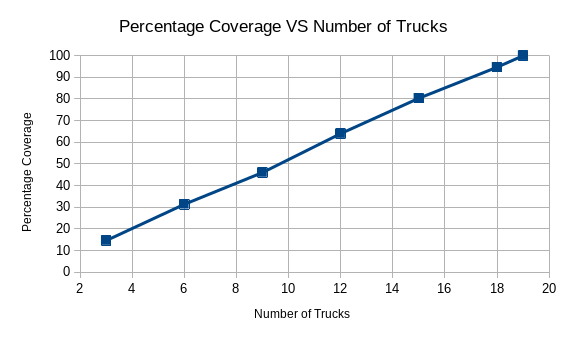
\includegraphics[width=\linewidth]{coverage_VS_number_of_trucks.png}
        \caption{For the entire city}\label{figc1}
    \end{subfigure}%
    \begin{subfigure}{0.5\textwidth}
        \centering
        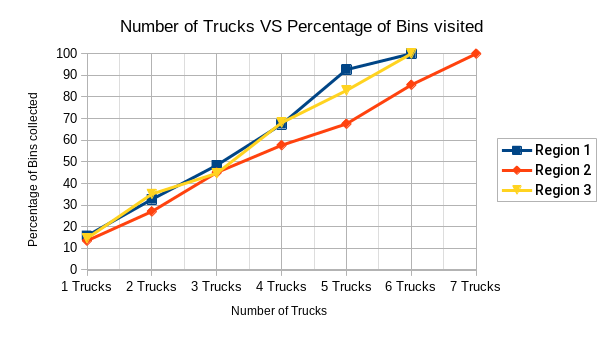
\includegraphics[width=\linewidth]{number_of_trucks_VS_bins_visited.png}
        \caption{Region-wise}\label{figc2}
    \end{subfigure}
    \caption{Effect of number of trucks on bin coverage}
    \label{fig3}
\end{figure}

 

\begin{figure}[H]
    \centering
    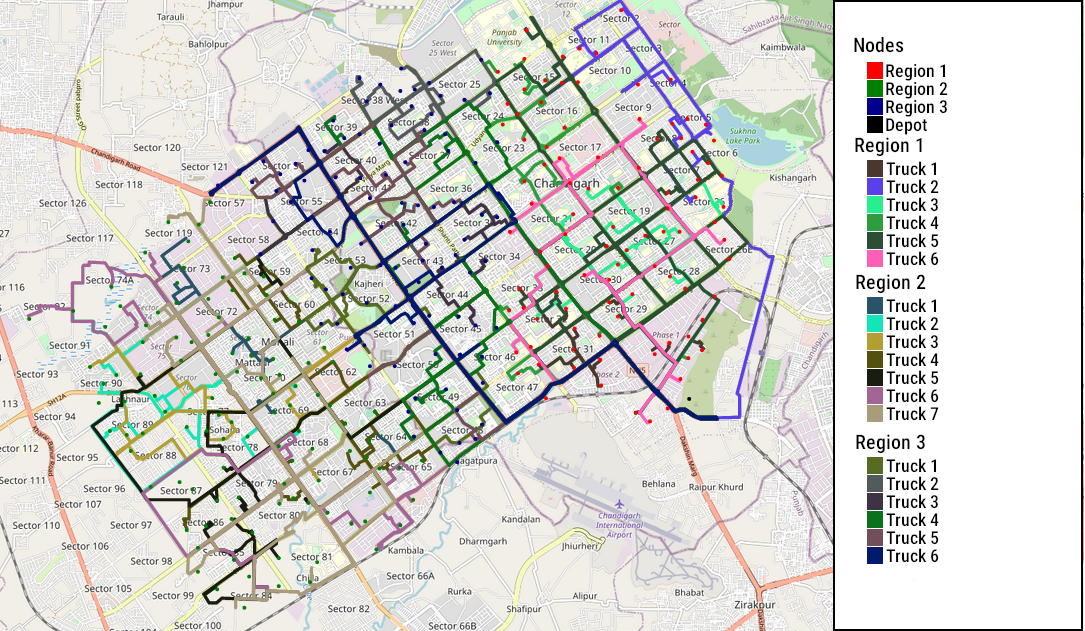
\includegraphics[scale=0.4]{Dynamic_weighted_unrestricted.png} % New Image added
    \caption{Realtime Unrestricted}\label{fig2}
\end{figure}


\subsubsection*{Case 3: Comparison of real-time with static route calculation}

Our base case of route calculation considers real time dynamics of waste (bin, truck) and truck's current position in real time. However, the existing collection system of the city is static. Hence, we compared the realtime route calculation model with the static by modifying the eq \eqref{eq12} as the constraint will be just less than 100, as shown in \eqref{eq12x}. In equation \eqref{eq2} and Eq \eqref{eq3} instead of \textit{st}, the beginning nodes will always be 0 \eqref{eq2x}\eqref{eq3x}. 
\begin{equation}\label{eq12x}
    u_i\le 100
\end{equation}
\begin{equation}\label{eq2x}
    \sum_{j\in N}X_{0,j}=1 ; \forall j \in N
\end{equation}
\begin{equation}\label{eq3x}
    \sum_{j\in N}X_{j,0}=1 ; \forall j \in N
\end{equation}

The above constraints when implemented results in a fixed optimal route which doesn't change with the time. We executed the dynamic and static models for 1 truck per region. The comparison is represented in Table \ref{tab5}

\begin{table}[H]
    \centering
    \caption{Comparison of static and real-time optimization performance} \label{tab5}
    \vspace*{0.3cm}
    \begin{tabular}{|c|c|c|c|}
        \hline Case & Waste (Kg) & Distance (Km) & Percent Covered\\
        \hline \textit{Static}& 8996.88 & 798.13 & 40.33\%\\
        \hline \textit{Real-Time}& 8967.25 & 517.8 & 46.00\%\\
        \hline
    \end{tabular}
\end{table}

The routes (Figure \ref{fig4} and Figure \ref{fig5}) show the routes obtained for static and dynamic case for one truck. The outcomes demonstrate the consideration of dynamic variables on the routes which are different than the static model. 

\begin{figure}[H]
    \centering
    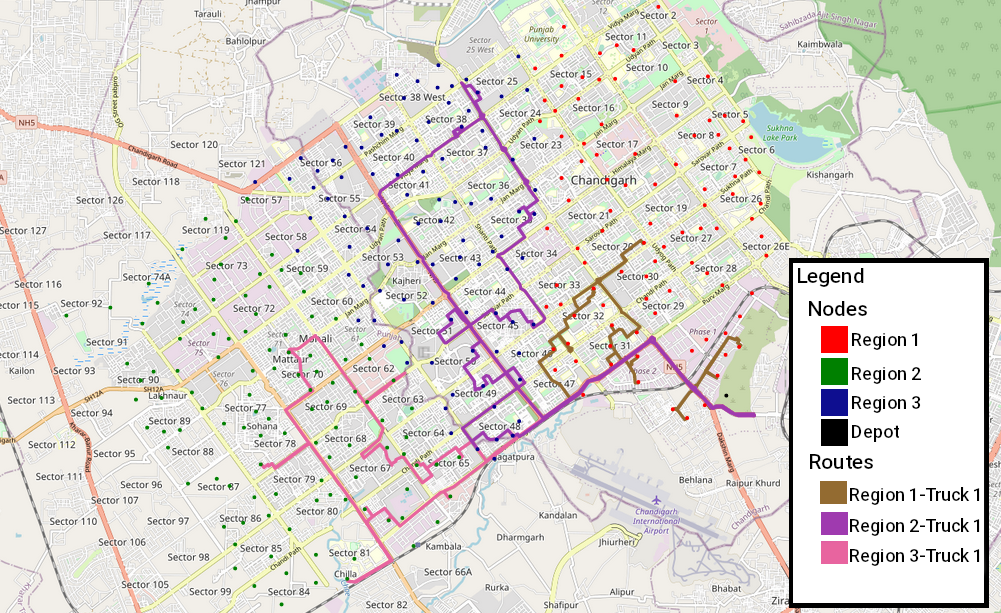
\includegraphics[scale=0.4]{Static_Unweighted.png} % Image changed here
    \caption{Routes for 1 truck per region as calculated by static optimization}\label{fig4}
\end{figure}
\begin{figure}[H]
    \centering
    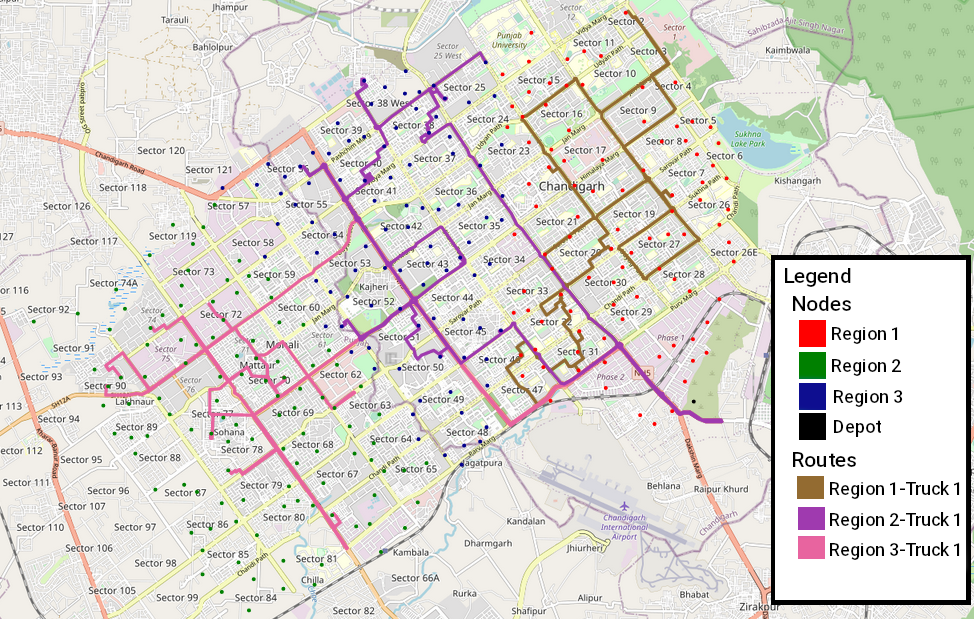
\includegraphics[scale=0.4]{Dynamic_weighted_1_Truck.png} % Image changed here
    \caption{Routes for 1 truck per region as calculated by real-time optimization}\label{fig5}
\end{figure}

We observe that the weight of the waste collected is nearly the same but the distance travelled by the trucks is smaller in the static case. This can be easily explained by the fact that, in essence, real-time method is just the static method applied repeatedly after certain intervals of time. Therefore, static gives one optimal route for the currently available data, but real-time has to do that each time the data is updated. It has to calculate new routes multiple times, even when the vehicle is already traversing the previous optimal route, and it also has to take the current position of the vehicle into consideration. This makes it inherently slightly more inefficient compared to the static method. 

This makes static optimization superior but only theoretically, because when applied in the real world, static has many disadvantages which are overcome by real-time optimization, such as adaptability and flexibility. In the static case, there is no accounting for new data. The initial route is the only route. This, consequently, also makes it unreliable. Real-time method, on the other hand, accounts for new data and creates new optimal routes taking it into consideration, making it very adaptable and reliable. Since real-time is just a modified and iterated version of the static method, the difference in computational power required between the two methods is not large. 

Therefore, for real life applications, real-time method is the superior method as it is able to deal with non-deterministic events that are common for ground use and adapt to them, giving an uninterrupted and reliable result.


 
\subsubsection*{Sensitivity Analysis of Weights}
In order to depict the effect of selected objective function weights on the waste  (\ref{figs1})  collected and the distance travelled by the collection trucks (\ref{figs2}), we performed a detailed sensitivity analysis. The Figures indicate that wights had highly non linear influence on the total distance travelled collected than the garbage collected. We normalized the distance and garbage collected values for their comparison (see \ref{figs}). From the graph it can be observed that the weight combinations such as W1=0.9,W2=0.1; W1=0.4,W2=0.6 can be reasonably good for maximizing the collection of waste at minimum distance cost (W1=0.9,W2=0.1). The outcome is also inline with our selected weights. The analysis as a decision making tool can help  in selecting the best weights for desired scenarios.

\begin{figure}[H]
    \centering
    \begin{subfigure}{0.5\textwidth}
        \centering
        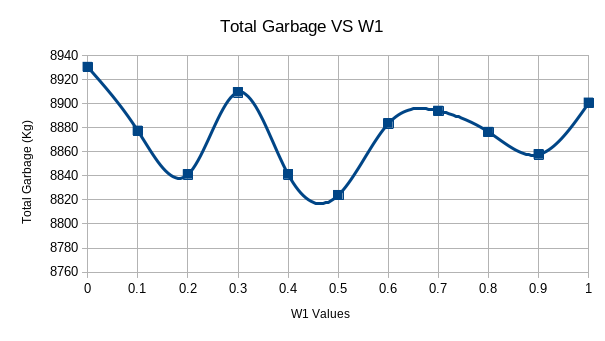
\includegraphics[width=\linewidth]{Total_Garbage_VS_W1_3_Trucks.png}
        \caption{Waste vs $w_1$}\label{figs1}
    \end{subfigure}%
    \begin{subfigure}{0.5\textwidth}
        \centering
        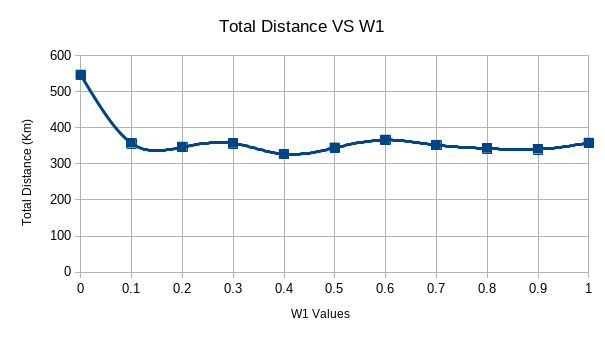
\includegraphics[width=\linewidth]{Total_Distance_VS_W1_3_Trucks.png}
        \caption{Distance vs $w_1$}\label{figs2}
    \end{subfigure}
    \caption{Effect of weight on waste and distance for 3 trucks per region}
    \label{figsz}
\end{figure}

\begin{figure}[H]
    \centering
    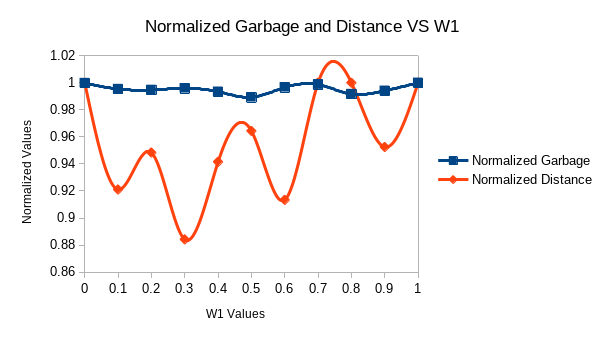
\includegraphics[scale=0.6]{Distance and Garbage Normalized VS W1.png}
    \caption{Normalized weight sensitivity graph}\label{figs}
\end{figure}



\section{Discussion and Policy Suggestions}

The collection of waste is a highly visible and important municipal service that involves large expenditures. Waste collection problems are, however, one of the most difficult operational problems to solve.

\textcolor{blue}{Having more trucks at your disposal is a matter of resources, and for a resource constrained region, their availability of trucks may not be sufficient for the amount of waste generated. That will, unless overcome by alternate methods such as multiple collection runs per vehicle, will lead to subpar waste collection, as shown by the data. However, those alternate methods are beyond the scope of the current work.}

One of the most noticeable observations that can be derived from the results is the weights attached to the two objectives in the objective function. In this case, the distance traveled was computed to be the main factor which must be considered when solving the objective function for the optimal solution. The waste collected appears to be almost completely irrelevant in this case. While this may look like an anomaly, this is solely due to the fact that this is a resource constrained operation. The trucks  have to continue their runs until they are full. Therefore, in the end, the amount of waste collected will always be equal to the maximum capacity, hence rendering maximizing the waste collected objective irrelevant.

However, we must keep in mind that this will not always be the case. In a case where the resources, that is, the trucks are more than sufficient to cover the demand, the weight for the objective to maximize waste collected will be greater. The more is the resource greater than the requirement, the greater the weight of that objective will be.

We also observe that the distance travelled in the case of real-time optimization is greater than that of static one. It is due to the fact the optimal routes are calculated multiple times with different starting points based on the truck's current location. This makes the resultant route slightly more inefficient when compared to the initial calculation. This is an unavoidable effect of recalculating the routes and not a problem with the algorithm as the path that is already been travelled is not considered by the newly calculated route, hence the resultant route is longer than the initial optimal route

We have selected the city of Chandigarh as the base location for paper because while it is our goal to focus on resource constrained regions for route optimization for waste collection, we also want to make it general enough so that with a few tweaks, the same method can also be scaled to be used for more developed regions and cities. Chandigarh was found to be the most suitable choice as it is the perfect blend of the two goals that we have: it is a well-planned city and still retains some of the characteristics of a developing nation.

Our program, once the initial setup of the nodes and the distance between two nodes is done, can efficiently and quickly calculate the optimal route that should be followed by a collection vehicle, whether once per run or in real time. Unlike the currently used systems that are either controlled manually or use general GPS systems to do their collection runs, our process is capable of:
\begin{itemize}
    \item Vastly improved performance in terms of distance travelled
    \item Smart bins further reduce the distance travelled by removing the need to visit redundant nodes
    \item We have used linear programming which is a simple yet novel approach to this problem and it is not too mathematically complex
    \item Our program is able to calculate new paths according to new data in real-time which is much more flexible than the systems currently being used in most places
    \item We also calculated the effects of resource availability on the overall performance and can further suggest the minimum amount of resources that would be sufficient for the operation.
\end{itemize}

For real world application of this method, the suggested policy would be to first use the software to calculate the current capabilities of the resources that are available, then apply the algorithm to utilize those resources, namely trucks, to their maximum potential and efficiency. If needed, how much more resources are needed to sufficiently cover the city in question can also be calculated by the software, and the results can be used as data for the requisition request of more resources.

\section{Conclusion}
We have achieved most of our core goals of optimizing waste collection with a focus on resource constrained societies. We were able to devise a method to use the available resources as efficiently as possible and at the same time ensure that the method also remains viable in more developed regions if scaled accordingly. Yet there still were things that we were not able to implement in our current endeavour. 

In our process, we divide the total number of nodes into specific clusters depending upon the resources that we have. These clusters are called regions and in the current version, vehicles assigned to each cluster are completely independent of the points in another cluster, and will not collect from a node from another cluster even when it is more efficient to do so. 

These can be taken as goals for future forays into this field to overcome the current limitations of our work. Scopes for future development may focus on improving upon our works by integrating more detailed street data like street signs, one-way roads and using the additional parameters as factors to provide a more street accurate route tailored for a specific region.

Future works may also focus on the effects different sets of weights may have on the results of the objective function for different granular levels of resource constraint. In our current work, we have focused solely on the best weights for one specific case. So further research can be done to find a more concrete relationship between weights, results and resource availability. 

In our current method of real time route calculation, our algorithm does not consider the route already travelled when calculating the new routes for new data. This leads to some degree of inefficiency in the optimization process and is also a viable topic for further work in this field.
\bibliographystyle{ieeetr}

\bibliography{citation}
\end{document}